\documentclass[11pt,a4paper]{article}
\usepackage[margin=2.5cm]{geometry}
\usepackage{booktabs}
\usepackage{graphicx}
\usepackage{xcolor}
\usepackage{hyperref}
\usepackage{enumitem}
\usepackage{titlesec}
\usepackage{fancyhdr}
\usepackage{microtype}
\usepackage{parskip}
\usepackage{fontspec}
\usepackage{polyglossia}
\usepackage{amsmath}
\usepackage{amssymb}

\setmainlanguage{english}
\setotherlanguage{hebrew}
\newfontfamily\hebrewfont{DejaVu Sans}[Script=Hebrew]

\hypersetup{colorlinks=true, linkcolor=blue, urlcolor=blue}

\pagestyle{fancy}
\fancyhf{}
\rhead{Knesset Protocol Journal Project}
\lhead{Step 5 --- Linking Baseline}
\rfoot{Page \thepage}
\lfoot{Tomer Morad, Or Israeli, Yoel Marko --- June 2026}

\titleformat{\section}{\large\bfseries}{\thesection.}{0.6em}{}[\titlerule]
\titleformat{\subsection}{\normalsize\bfseries}{\thesubsection}{0.6em}{}

\begin{document}

\begin{center}
  {\LARGE \textbf{Streaming Subject Linking: Similarity Threshold Baseline}}\\[0.3em]
  {\large Step 5 --- Task 2a: how far does cosine similarity alone get us?}\\[0.6em]
  {\normalsize Tomer Morad \quad Or Israeli \quad Yoel Marko}\\
  {\normalsize June 2026}
\end{center}

\vspace{0.5em}

% ----------------------------------------------------------------------
\section{Objective}

\textbf{Task 2} of the Knesset Protocol Journal Project is \emph{streaming subject linking}:
as protocol spans arrive chronologically, classify each as
\textbf{LINK} (belongs to an existing journal entry) or \textbf{NEW} (opens a fresh entry).

This step implements and evaluates the simplest possible baseline: a \textbf{cosine similarity
threshold} over the best representations from Steps 3--4.  No LLM is involved.  The goals are:
\begin{enumerate}[noitemsep]
  \item Establish a quantitative floor for linking performance.
  \item Characterize the precision--recall trade-off, especially the
        \textbf{false-merge rate} (FMR), which is asymmetrically costly: a false merge
        irreversibly conflates two distinct legislative matters in the journal.
  \item Determine whether the baseline is sufficient or whether an LLM verifier is needed.
\end{enumerate}

% ----------------------------------------------------------------------
\section{Method}

\subsection{Task setup}

Each of the 198 clean spans has a gold canonical topic label (Step 1).  28 topics
recur across $\ge 2$ protocols (105 spans); 93 topics appear exactly once.

\textbf{Gold labels for the streaming decision:}
\begin{itemize}[noitemsep]
  \item A span's \emph{first} chronological occurrence $\to$ gold = \textbf{NEW}.
  \item All subsequent occurrences of the same topic $\to$ gold = \textbf{LINK}.
\end{itemize}
This yields 77 LINK instances and 121 NEW instances across the 198 spans.

\subsection{Decision rule}

Let $R = \{r_1, \ldots, r_m\}$ be the current set of journal-entry representatives
(one embedding per entry, initialized to the first span seen for that entry).
For an incoming span $s$:
\[
  \hat{y}(s; \theta) =
  \begin{cases}
    \text{LINK to } \arg\max_j \cos(s, r_j) & \text{if } \max_j \cos(s, r_j) \ge \theta,\\
    \text{NEW} & \text{otherwise.}
  \end{cases}
\]
We sweep $\theta \in [0, 1]$ in steps of 0.005 to obtain full precision--recall and
false-merge-rate curves.

\subsection{Evaluation modes}

\paragraph{Pairwise (oracle upper bound).}
For all $\binom{105}{2}$ ordered pairs within the recurring subset, predict LINK if
$\cos(i,j) \ge \theta$.  This assumes perfect access to all past spans and is the ceiling
on what the similarity function can achieve.

\paragraph{Streaming simulation (realistic).}
Process all 198 spans in chronological order.  Journal entries are represented by the
first span seen for each cluster (no centroid update).  Errors propagate: a wrong link
joins two clusters permanently.

\subsection{Representations tested}

\begin{center}
\begin{tabular}{lll}
\toprule
\textbf{Name} & \textbf{Construction} & \textbf{Why} \\
\midrule
\texttt{e5\_k1}    & ABTT $k=1$ on \texttt{e5}-large & Best AUC (0.899) from Step 3 \\
\texttt{alephbert\_k2} & ABTT $k=2$ on AlephBERT & Best ARI$_\text{agg}$ from Step 3 \\
\texttt{hybrid}$_{\alpha=0.6}$ & $0.6 \cdot S_\text{tfidf} + 0.4 \cdot S_\text{alephbert\_k2}$ & Best precision-priority from Step 4 \\
\bottomrule
\end{tabular}
\end{center}

% ----------------------------------------------------------------------
\section{Results}

\subsection{Pairwise evaluation}

\begin{center}
\begin{tabular}{lcccc}
\toprule
\textbf{Representation} & \textbf{AUC} & \textbf{Best F1} & \textbf{$\theta$} & \textbf{F1 (FMR$\le5\%$)} \\
\midrule
\textbf{\texttt{e5\_k1}} & \textbf{0.899} & \textbf{0.531} & 0.33 & \textbf{0.503} \\
\texttt{alephbert\_k2}   & 0.887 & 0.472 & 0.32 & 0.464 \\
\texttt{hybrid}$_{\alpha=0.6}$ & 0.879 & 0.463 & 0.20 & 0.463 \\
\bottomrule
\end{tabular}
\end{center}

\noindent\texttt{e5\_k1} leads on all metrics.  At the precision-priority operating point
(FMR$\le5\%$) the pairwise F1 drops only slightly (0.531 $\to$ 0.503 at $\theta=0.26$),
suggesting the score distributions are reasonably well-separated in the oracle setting.

\begin{center}
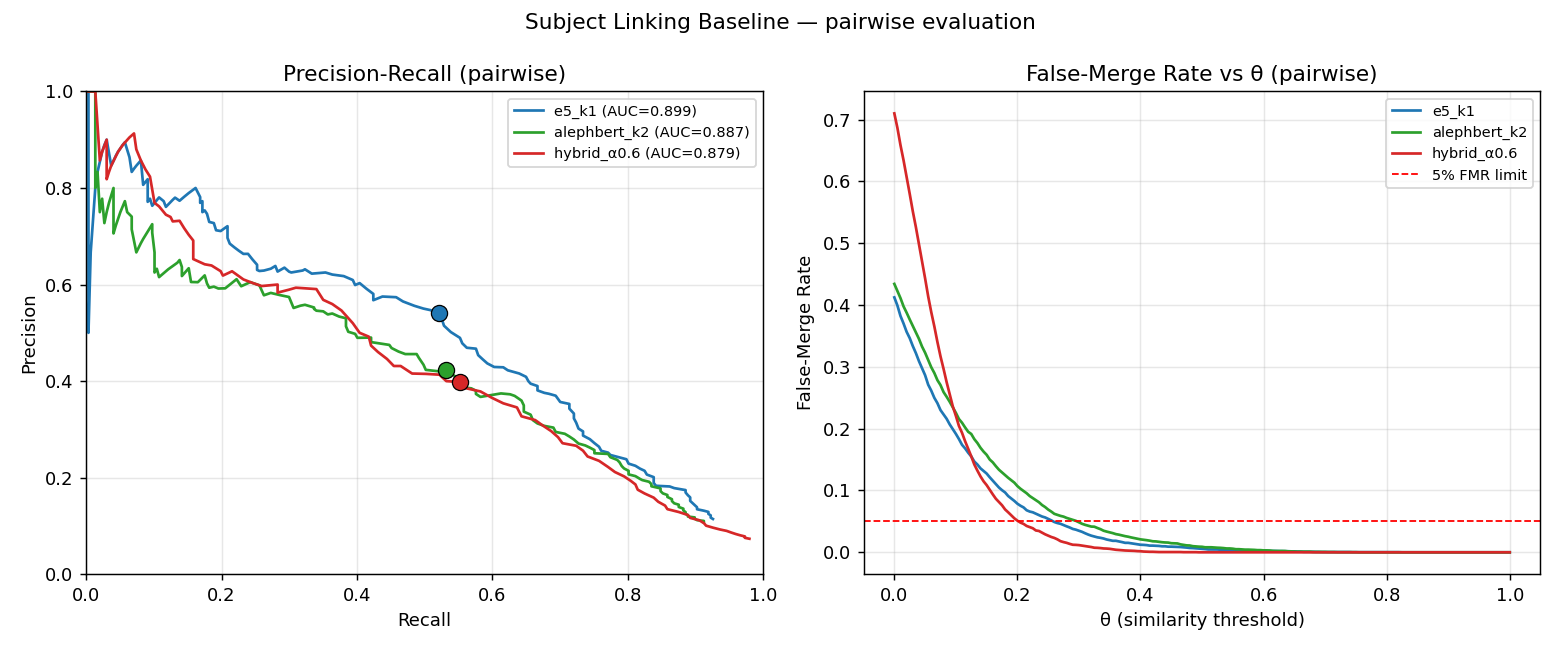
\includegraphics[width=\textwidth]{../outputs/pr_curves_pairwise.png}
\end{center}
\noindent Left: precision--recall curves (filled circles = F1-optimal threshold per model).
Right: false-merge rate vs.\ $\theta$ (dashed line = 5\% FMR budget).

\subsection{Streaming simulation}

\begin{center}
\begin{tabular}{lccccc}
\toprule
\textbf{Representation} & \textbf{Best F1} & \textbf{$\theta$} & \textbf{P} & \textbf{R}
  & \textbf{F1 (FMR$\le5\%$)} \\
\midrule
\textbf{\texttt{e5\_k1}}    & \textbf{0.411} & 0.52 & 0.419 & 0.403 & 0.092 \\
\texttt{alephbert\_k2}      & 0.342 & 0.62 & 0.500 & 0.260 & 0.114 \\
\textbf{\texttt{hybrid}$_{\alpha=0.6}$} & 0.377 & 0.36 & 0.426 & 0.338 & \textbf{0.196} \\
\bottomrule
\end{tabular}
\end{center}

\begin{center}
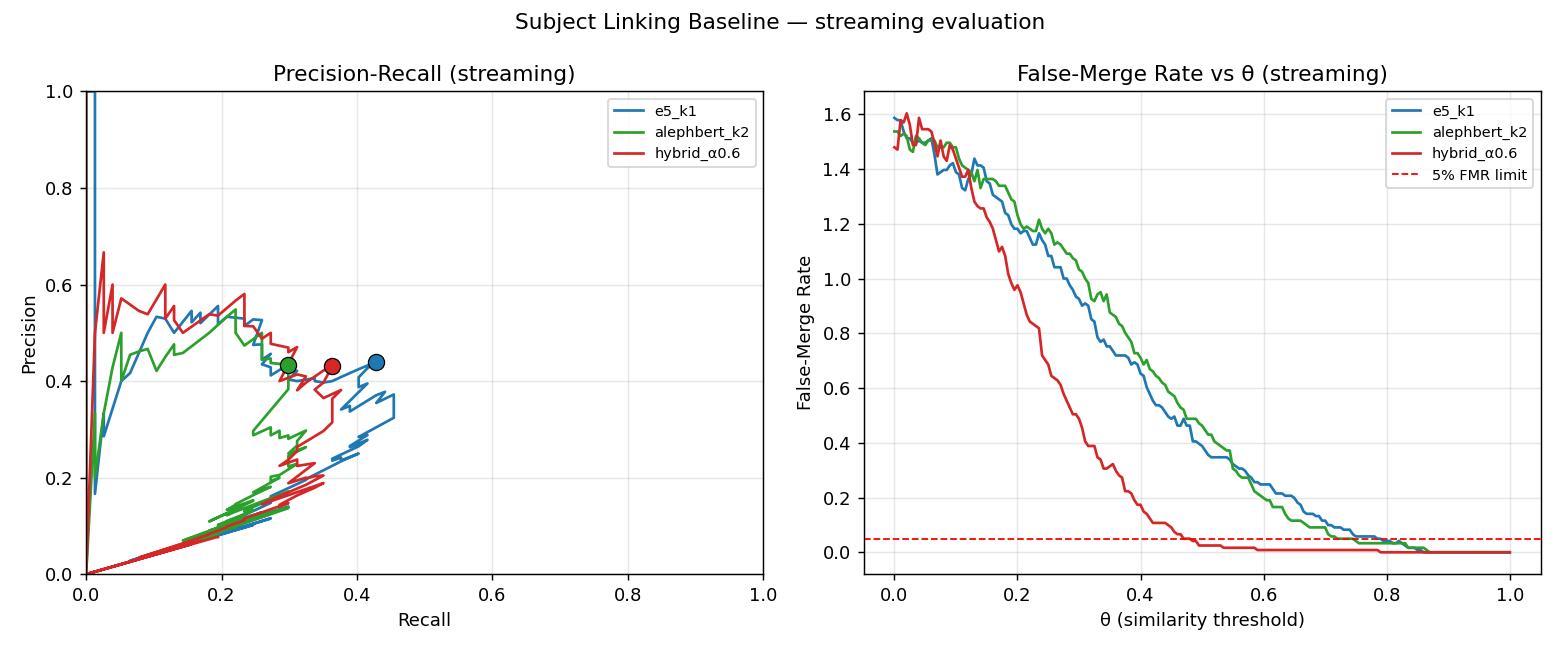
\includegraphics[width=\textwidth]{../outputs/pr_curves_streaming.png}
\end{center}
\noindent Same layout as above but for the streaming simulation.

\subsection{Analysis of the pairwise--streaming gap}

The best pairwise F1 (0.531) drops to 0.411 in the streaming simulation for \texttt{e5\_k1}
--- a gap of 0.12.  This is caused by the \textbf{first-span-representative} approximation:
the first occurrence of a topic is often an introductory or procedural discussion whose
embedding is not representative of the full legislative matter.  Later spans, which discuss
the matter in depth, are compared against this impoverished representative.

\subsection{The anti-duplication operating point}

At the precision-priority constraint (FMR$\le5\%$), streaming recall collapses:
\begin{itemize}[noitemsep]
  \item \texttt{e5\_k1}: F1 = 0.092 at $\theta=0.79$ --- only the most obvious recurring
        spans are linked.
  \item \texttt{hybrid}$_{\alpha=0.6}$: F1 = 0.196 at $\theta=0.47$ --- TF-IDF's bill-number
        precision prevents false merges at a lower threshold, recovering more recall.
\end{itemize}

\noindent This is the central finding: \textbf{no single threshold satisfies both the
anti-duplication constraint (FMR$\le5\%$) and useful recall (F1$\ge0.3$)} using similarity
alone.  The distributions of same-topic and different-topic cosine similarities overlap too
much in the streaming setting for a threshold to cleanly separate them.

% ----------------------------------------------------------------------
\section{Takeaways}

\begin{itemize}[noitemsep]
  \item \textbf{Pairwise AUC is strong} (0.899) but does not translate to high streaming F1.
        The bottleneck is the first-span-representative, not the similarity function itself.
  \item \textbf{The similarity baseline is insufficient for anti-duplication deployment.}
        At FMR$\le5\%$, the best streaming F1 is 0.196.  A journal system using only
        similarity thresholds would either miss most recurrences or create false merges.
  \item \textbf{Hybrid $\alpha=0.6$ is the best precision-priority choice} because TF-IDF
        bill-identifier signal is discriminative at the precision-critical margin.
  \item The gap between pairwise and streaming performance points directly to
        \textbf{centroid-based entry representation} as the quickest engineering fix,
        and to \textbf{LLM-based verification} as the path to production-quality linking.
\end{itemize}

% ----------------------------------------------------------------------
\section{Recommended Operating Points}

\begin{center}
\begin{tabular}{lll}
\toprule
\textbf{Use case} & \textbf{Representation} & \textbf{$\theta$} \\
\midrule
Recall-maximizing (false merges acceptable) & \texttt{e5\_k1} & 0.33 \\
Precision-priority journal (FMR$\le5\%$) & \texttt{hybrid}$_{\alpha=0.6}$ & 0.47 \\
Retrieval pre-filter for LLM verifier & \texttt{e5\_k1} & rank, don't threshold \\
\bottomrule
\end{tabular}
\end{center}

% ----------------------------------------------------------------------
\section{Future Directions}

\begin{enumerate}[leftmargin=1.4em]
  \item \textbf{LLM retrieve-then-verify (Task 2b).}  Use \texttt{e5\_k1} to retrieve
        the top-$K$ journal candidates ($K=3$--$5$, $\theta=0.33$) and prompt a
        Hebrew-capable LLM to classify each as \emph{same} / \emph{related} / \emph{new}
        given the candidate's full prior timeline.  This is the critical next step.
  \item \textbf{Centroid-based entry representation.}  Replace the first-span representative
        with a running centroid over all ABTT-corrected embeddings linked to the entry.
        Expect to close a significant portion of the pairwise--streaming gap.
  \item \textbf{Annotated evaluation set.}  Manually label a stratified sample of span
        pairs for LINK / RELATED / NEW to enable three-class evaluation and remove
        reliance on topic-label proxy supervision.
  \item \textbf{Asymmetric threshold tuning.}  Calibrate separately on topics known to
        be legislatively similar (budget sub-items, closely related bills) vs.\ unrelated
        topics to narrow the hard overlap region.
\end{enumerate}

\vspace{1.5em}
\hrule
\vspace{0.4em}
{\small
\textbf{Artifacts (this step):}
\texttt{outputs/linking\_results.json},
\texttt{outputs/pr\_curves\_pairwise.png},
\texttt{outputs/pr\_curves\_streaming.png}.\\
\textbf{Code:} \texttt{code/linking\_baseline.py}.
}

\end{document}
